\section{Einleitung}

Der Einsatz von Kränen ist auf Baustellen unerlässlich, um schwere Lasten zu bewegen.
Aktuell erfordert das Anhängen dieser Lasten an den Kran manuelle Arbeit durch Bauarbeiter.
Dies ist besonders zeitaufwendig, wenn der Schwerpunkt der Last ungleichmässig verteilt ist 
und führt häufig dazu, dass die Last mehrmals abgesetzt und angehoben werden muss, um sie 
korrekt auszurichten. Dies verursacht erhebliche Wartezeiten für andere Teammitglieder. 
Die Firma Ludwig System hat eine automatische Traverse entwickelt, die das Ausrichten und 
Positionieren der Last erleichtert, jedoch muss auch mit dieser aktuellen Version ein Mitarbeiter 
die Last manuell an die Traverse anhängen.

\begin{figure}[H]
    \centering
    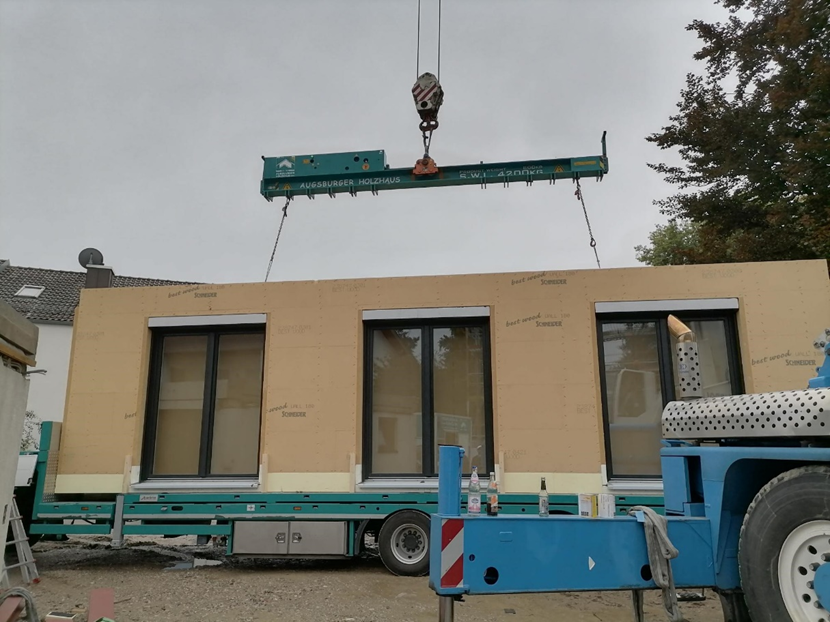
\includegraphics[width=\linewidth]{traverse.png}
    \caption{Ludwig Traverse im Einsatz}
\end{figure}

Die nächste Generation der Traverse zielt darauf ab, den Prozess der Lastenaufhängung zu automatisieren.
Ludwig System arbeitet derzeit intensiv an dieser Entwicklung und hat bereits Prototypen eines Greifarms 
erstellt, der dazu bestimmt ist, die Anschlagspunkte automatisch zu heben. Ein entscheidender Schritt in diesem 
Prozess ist die präzise Berechnung der Position dieser Anschlagspunkte.

Auf den ersten Blick erscheinen moderne Lösungen aus dem Bereich des maschinellen Lernens als ideal für diese Aufgabe. 
Jedoch besteht die Herausforderung darin, dass für das Training eines effektiven Modells eine umfangreiche Menge an Daten 
benötigt wird, die derzeit noch nicht ausreichend verfügbar ist. Zusätzlich erfordert die Anwendung solcher Technologien weiterführende 
Forschungen, um aus den erkannten Anschlagspunkten die Entfernung und Ausrichtung relativ zur Kamera zu bestimmen. Diese Berechnungen werden 
noch komplexer, wenn die Anschlagspunkte in verschiedenen Dimensionen vorliegen, was eine zusätzliche Anpassung und Verfeinerung der Algorithmen 
erfordert.

Ein weiterer Ansatz ist die Verwendung von Passmarkern. Diese Marker haben den Vorteil, dass sie in standardisierten Grössen verfügbar sind, was 
ihre Erkennung erleichtert \cite{astrobee2023}. Durch die Analyse der Eckpunkte eines Markers kann die Position relativ zur Kamera bestimmt werden 
\cite{localizationSystem}. Zusätzlich ermöglicht die Kodierung einer eindeutigen ID auf dem Marker die Feststellung seiner Ausrichtung. Theoretisch
erlaubt dies dem Kranführer, die Traverse präzise auszurichten. Der Einsatz solcher Markierungssysteme wird bereits in der Robotik erfolgreich zur 
Positionsbestimmung von Objekten genutzt, was deren Effektivität und Zuverlässigkeit unterstreicht \cite{localizationSystem}.

Die Arbeiten von \cite{yong_object_2023} und \cite{zhou_image-based_2021} zeigen, dass mithilfe von Machine-Learning-Methoden Objekte erfolgreich identifiziert werden können.
Da uns jedoch die nötigen Daten fehlen, um KI zur Bestimmung von Anschlagpunkten einzusetzen, fokussieren wir uns in dieser Arbeit auf Fiducial Marker. Diese bieten den Vorteil, 
dass ihre Ausrichtung und Grösse im Voraus festgelegt werden können, was Berechnungen vereinfacht. Für unsere Anwendung haben wir AprilTags gewählt, da sie in Vergleichstests höhere 
Genauigkeiten als AruCo-Marker erzielen. Um die Position des Anschlagpunktes zu bestimmen nutzen wir ein Kreuzmuster aus vier AprilTags, bei dem der Anschlagpunkt zentral in der Mitte liegt.
Tests und ein Prototyp zeigen, dass die Abweichungen innerhalb der vom Kunden geforderten Toleranzgrenzen liegen, wodurch unser Ansatz eine praktikable Lösung darstellt.

\begin{figure}[H]
    \centering
    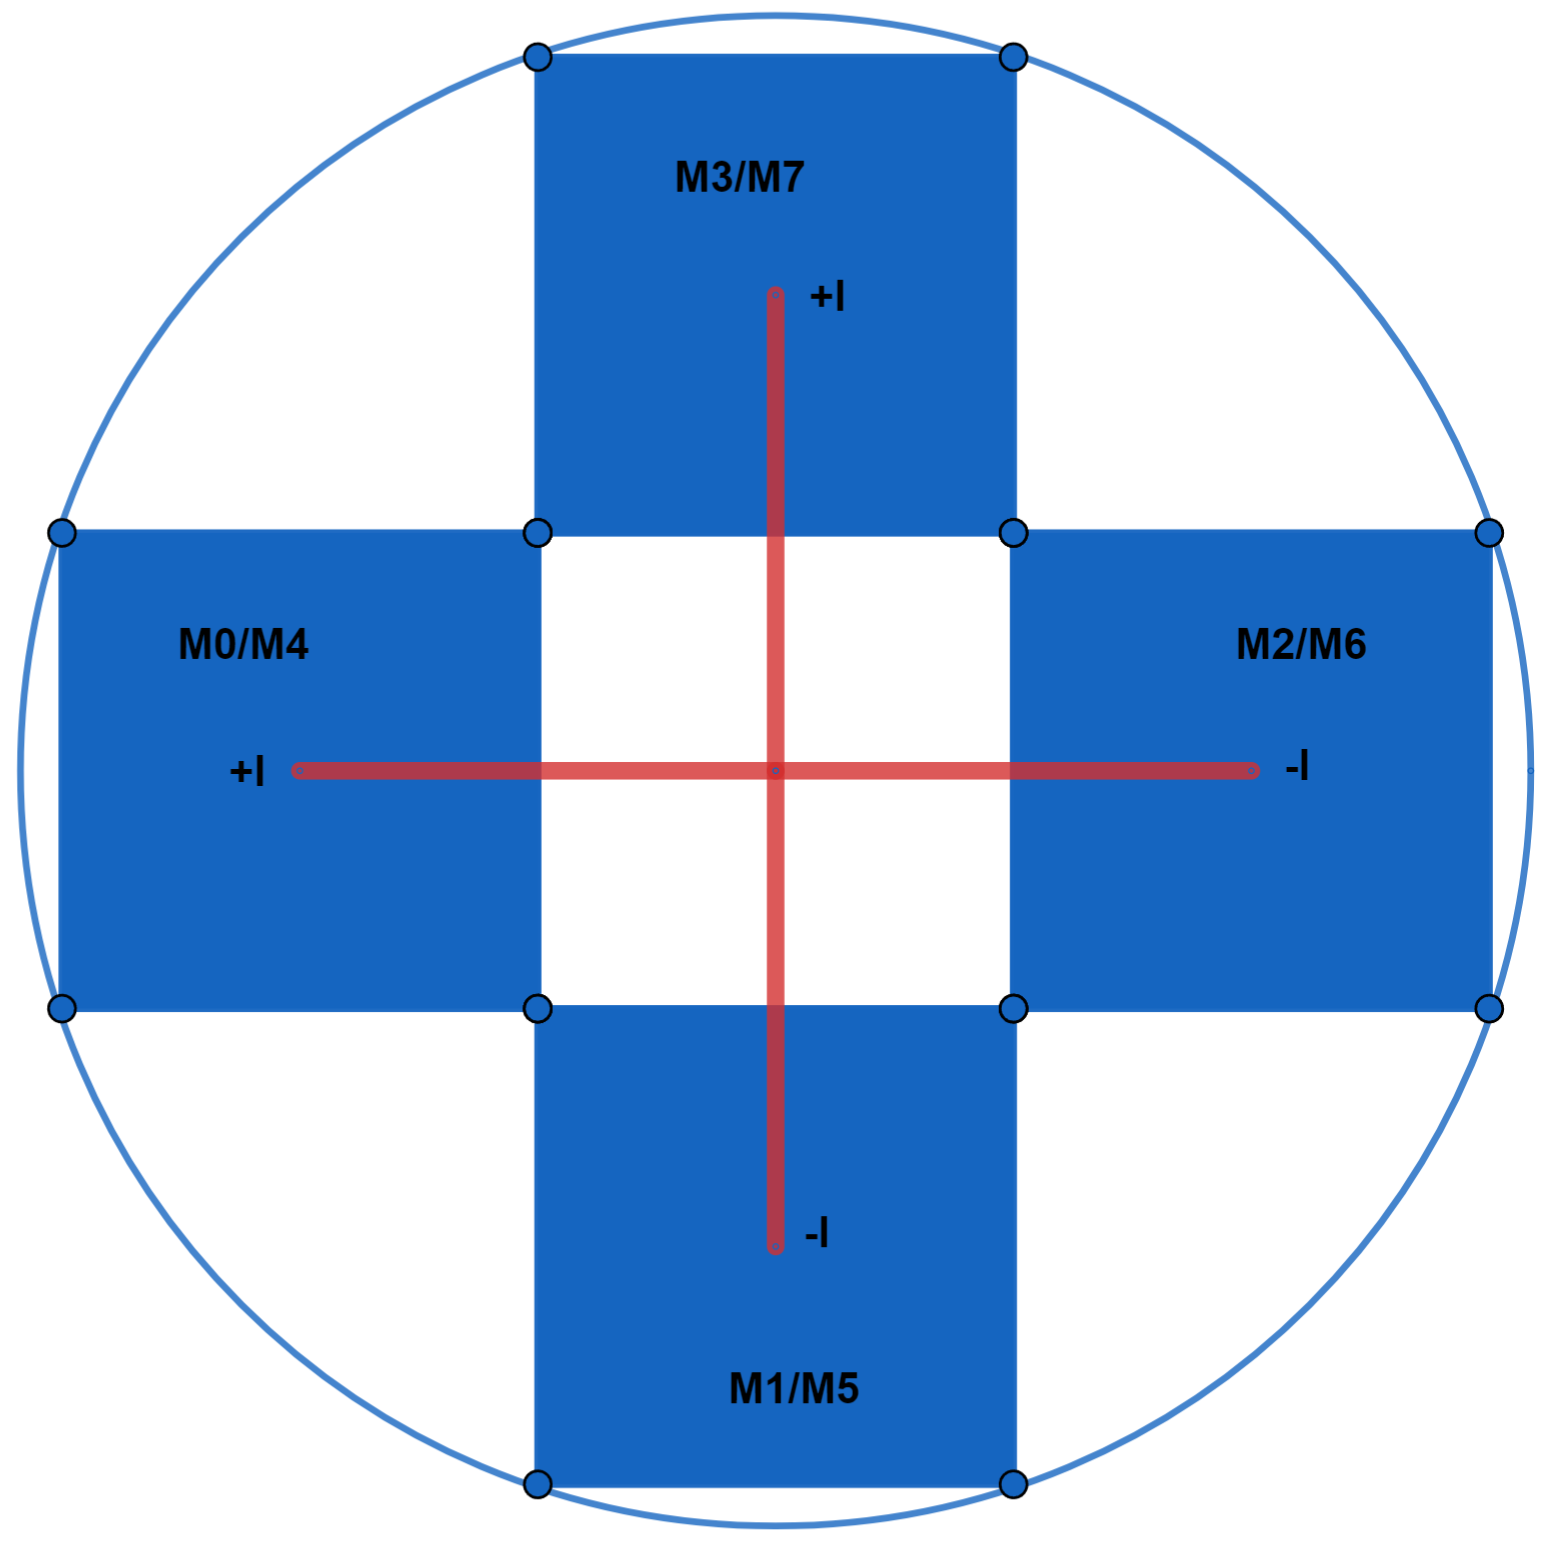
\includegraphics[width=0.5\linewidth]{graphics/marker_anordnung.png}
    \caption{Kreuzmuster zur Positionsbestimmung}
\end{figure}


In den folgenden Kapiteln schaffen wir zunächst eine Grundlage, um das Problem und unsere Lösung besser zu verstehen. Anschliessend 
widmen wir uns Projekten, die ähnliche Herausforderungen bereits behandelt haben.

Darauf aufbauend präsentieren wir unsere Konzepte zunächst theoretisch, bevor wir zur praktischen Implementierung 
übergehen. Abschliessend stellen wir unsere Ergebnisse vor, diskutieren mögliche Alternativen zur Problemlösung und 
zeigen auf, wie wir unsere Ansätze weiter verbessern könnten.


